
\lecture{The t-distribution}{t-table}
\section{The t-distribution}

\title{The $t$-Distribution}
\subtitle{When you only know the sample standard deviation}

%\author{Kelly Black}
%\institute{Clarkson University}
\date{28 March 2013}

\begin{frame}
  \titlepage
\end{frame}

\begin{frame}
  \frametitle{Outline}
  \tableofcontents[pausesection,hideothersubsections,sectionstyle=show/hide]
\end{frame}


\subsection{Clicker Quiz}


\iftoggle{clicker}{%
  \begin{frame}{Clicker Quiz}

    The volume for a stock is sampled on twenty randomly chosen
    days. The sample mean for the volume is 2.65 million shares per
    day. The standard deviation is 0.85 million shares per day. What
    is the 95\% confidence interval for the estimation of the mean
    number of shares traded?

    \vfill

    \begin{tabular}{l@{\hspace{3em}}l@{\hspace{3em}}l@{\hspace{3em}}l}
      A: 2.34 - 2.96 million shares  & B: 2.28 to 3.02 million shares 
    \end{tabular}

    \vfill
    \vfill
    \vfill

  \end{frame}
}


\begin{frame}{Problem!}

  We do not know $\sigma$ in practice!

  What do we do?
  
\end{frame}





\subsection{The $t$-Distribution}


\begin{frame}
  \frametitle{$t$-Distribution}

  \begin{definition}[$t$-Distribution]

    A $t$-distribution is the distribution associated with the expression
    \begin{eqnarray*}
      t &  = & \frac{\bar{x}-\mu}{\lp \frac{s}{\sqrt{n}} \rp}.
    \end{eqnarray*}

    The number of ``\textit{degrees of freedom}'' is $n-1$.
    
  \end{definition}

  Because the distribution depends on $n-1$ means that we need a
  different table for every possible value of $n$. Instead we just
  have a table for the critical values for some values of $n$.
  

\end{frame}

\begin{frame}{The $t$-distribution}

  \only<1>{\centerline{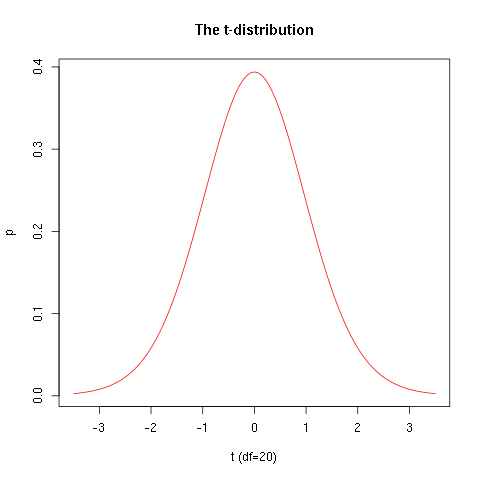
\includegraphics[width=5cm]{img/tdistExample}}}
  \only<2>{\centerline{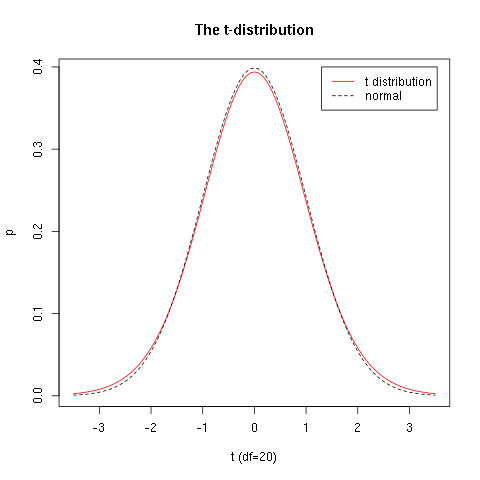
\includegraphics[width=5cm]{img/tdistComparison}}}
  
\end{frame}


\begin{frame}
  \frametitle{Comparison}

  \begin{columns}
    \column{0.5\textwidth}
    Normal Distribution:
    \begin{eqnarray*}
      z &  = & \frac{\bar{x}-\mu}{\lp \frac{\sigma}{\sqrt{n}} \rp}.
    \end{eqnarray*}

    \column{0.5\textwidth}
    $t$-Distribution:
    \begin{eqnarray*}
      t &  = & \frac{\bar{x}-\mu}{\lp \frac{s}{\sqrt{n}} \rp}, \\
      df & = & n-1.
    \end{eqnarray*}

  \end{columns}

  \vfill

    \only<2->
    {

      \begin{center}
        The algebra and concepts are exactly the same!

        The only difference is $\sigma$ vs. $s$ and $df=n-1$.
      \end{center}
    }

    \vfill
  

\end{frame}


\begin{frame}{The $t$-distribution Table}

  The $t$-distribution table is different from the normal distribution
  table. The issue is that the distribution is different for every
  value of the number of degrees of freedom.

  \vfill

  The table only has \textit{critical values}.

  \centerline{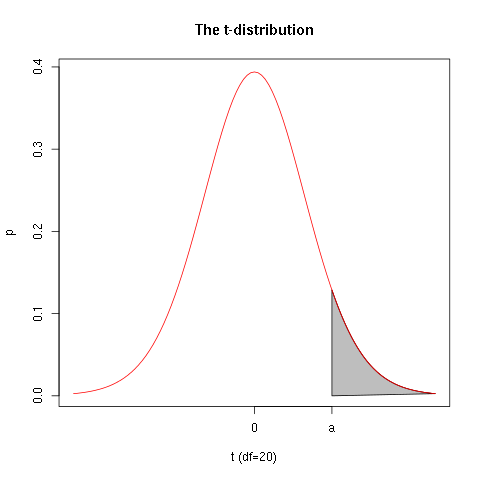
\includegraphics[width=5cm]{img/tdistTable}}

  That is, given the area in grey and the number of degrees of
  freedom, the table gives the value of $a$.
  
\end{frame}


\begin{frame}
  \frametitle{The Table}
  {
\fontencoding{T1}
\fontfamily{pcr}
\fontseries{m}
\fontshape{n}
\fontsize{5pt}{5pt}
\selectfont

\begin{tabular}{l|llllllllll}
 & 0.1&0.05&0.025&0.01&0.005&0.001&0.00005\\ \hline
 1 & 3.078 & 6.314 & 12.706 & 31.821 & 63.657 & 318.309 & 636.619 \\ 
 2 & 1.886 & 2.920 & 4.303 & 6.965 & 9.925 & 22.327 & 31.599 \\ 
 3 & 1.638 & 2.353 & 3.182 & 4.541 & 5.841 & 10.215 & 12.924 \\ 
 4 & 1.533 & 2.132 & 2.776 & 3.747 & 4.604 & 7.173 & 8.610 \\ 
 5 & 1.476 & 2.015 & 2.571 & 3.365 & 4.032 & 5.893 & 6.869 \\ 
[5pt]
 6 & 1.440 & 1.943 & 2.447 & 3.143 & 3.707 & 5.208 & 5.959 \\ 
 7 & 1.415 & 1.895 & 2.365 & 2.998 & 3.499 & 4.785 & 5.408 \\ 
 8 & 1.397 & 1.860 & 2.306 & 2.896 & 3.355 & 4.501 & 5.041 \\ 
 9 & 1.383 & 1.833 & 2.262 & 2.821 & 3.250 & 4.297 & 4.781 \\ 
10 & 1.372 & 1.812 & 2.228 & 2.764 & 3.169 & 4.144 & 4.587 \\ 
[5pt]
11 & 1.363 & 1.796 & 2.201 & 2.718 & 3.106 & 4.025 & 4.437 \\ 
12 & 1.356 & 1.782 & 2.179 & 2.681 & 3.055 & 3.930 & 4.318 \\ 
13 & 1.350 & 1.771 & 2.160 & 2.650 & 3.012 & 3.852 & 4.221 \\ 
14 & 1.345 & 1.761 & 2.145 & 2.624 & 2.977 & 3.787 & 4.140 \\ 
15 & 1.341 & 1.753 & 2.131 & 2.602 & 2.947 & 3.733 & 4.073 \\ 
[5pt]
16 & 1.337 & 1.746 & 2.120 & 2.583 & 2.921 & 3.686 & 4.015 \\ 
17 & 1.333 & 1.740 & 2.110 & 2.567 & 2.898 & 3.646 & 3.965 \\ 
18 & 1.330 & 1.734 & 2.101 & 2.552 & 2.878 & 3.610 & 3.922 \\ 
19 & 1.328 & 1.729 & 2.093 & 2.539 & 2.861 & 3.579 & 3.883 \\ 
20 & 1.325 & 1.725 & 2.086 & 2.528 & 2.845 & 3.552 & 3.850 \\ 
[5pt]
21 & 1.323 & 1.721 & 2.080 & 2.518 & 2.831 & 3.527 & 3.819 \\ 
22 & 1.321 & 1.717 & 2.074 & 2.508 & 2.819 & 3.505 & 3.792 \\ 
23 & 1.319 & 1.714 & 2.069 & 2.500 & 2.807 & 3.485 & 3.768 \\ 
24 & 1.318 & 1.711 & 2.064 & 2.492 & 2.797 & 3.467 & 3.745 \\ 
25 & 1.316 & 1.708 & 2.060 & 2.485 & 2.787 & 3.450 & 3.725 \\ 
[5pt]
26 & 1.315 & 1.706 & 2.056 & 2.479 & 2.779 & 3.435 & 3.707 \\ 
27 & 1.314 & 1.703 & 2.052 & 2.473 & 2.771 & 3.421 & 3.690 \\ 
28 & 1.313 & 1.701 & 2.048 & 2.467 & 2.763 & 3.408 & 3.674 \\ 
29 & 1.311 & 1.699 & 2.045 & 2.462 & 2.756 & 3.396 & 3.659 \\ 
30 & 1.310 & 1.697 & 2.042 & 2.457 & 2.750 & 3.385 & 3.646 \\ 
[5pt]
40 & 1.303 & 1.684 & 2.021 & 2.423 & 2.704 & 3.307 & 3.551 \\ 
50 & 1.299 & 1.676 & 2.009 & 2.403 & 2.678 & 3.261 & 3.496 \\ 
60 & 1.296 & 1.671 & 2.000 & 2.390 & 2.660 & 3.232 & 3.460 \\ 
120 & 1.289 & 1.658 & 1.980 & 2.358 & 2.617 & 3.160 & 3.373 \\ 
$\infty$ & 1.282 & 1.645 & 1.960 & 2.326 & 2.576 & 3.090 & 3.291 
\end{tabular}


}
\end{frame}


\begin{frame}{\small Example: Find $t^*$ value for $p(|t|>t^*)
\approx 0.01$ with 12 degrees of freedom.}
{\tiny First find the row corresponding to $df=12$.}

  {
\fontencoding{T1}
\fontfamily{pcr}
\fontseries{m}
\fontshape{n}
\fontsize{5pt}{5pt}
\selectfont

\begin{tabular}{l|llllllllll}
 & 0.1&0.05&0.025&0.01&0.005&0.001&0.00005\\ \hline
 1 & 3.078 & 6.314 & 12.706 & 31.821 & 63.657 & 318.309 & 636.619 \\ 
 2 & 1.886 & 2.920 & 4.303 & 6.965 & 9.925 & 22.327 & 31.599 \\ 
 3 & 1.638 & 2.353 & 3.182 & 4.541 & 5.841 & 10.215 & 12.924 \\ 
 4 & 1.533 & 2.132 & 2.776 & 3.747 & 4.604 & 7.173 & 8.610 \\ 
 5 & 1.476 & 2.015 & 2.571 & 3.365 & 4.032 & 5.893 & 6.869 \\ 
[5pt]
 6 & 1.440 & 1.943 & 2.447 & 3.143 & 3.707 & 5.208 & 5.959 \\ 
 7 & 1.415 & 1.895 & 2.365 & 2.998 & 3.499 & 4.785 & 5.408 \\ 
 8 & 1.397 & 1.860 & 2.306 & 2.896 & 3.355 & 4.501 & 5.041 \\ 
 9 & 1.383 & 1.833 & 2.262 & 2.821 & 3.250 & 4.297 & 4.781 \\ 
10 & 1.372 & 1.812 & 2.228 & 2.764 & 3.169 & 4.144 & 4.587 \\ 
[5pt]
11 & 1.363 & 1.796 & 2.201 & 2.718 & 3.106 & 4.025 & 4.437 \\ 
\rowcolor{red}12 & 1.356 & 1.782 & 2.179 & 2.681 & 3.055 & 3.930 & 4.318 \\ 
13 & 1.350 & 1.771 & 2.160 & 2.650 & 3.012 & 3.852 & 4.221 \\ 
14 & 1.345 & 1.761 & 2.145 & 2.624 & 2.977 & 3.787 & 4.140 \\ 
15 & 1.341 & 1.753 & 2.131 & 2.602 & 2.947 & 3.733 & 4.073 \\ 
[5pt]
16 & 1.337 & 1.746 & 2.120 & 2.583 & 2.921 & 3.686 & 4.015 \\ 
17 & 1.333 & 1.740 & 2.110 & 2.567 & 2.898 & 3.646 & 3.965 \\ 
18 & 1.330 & 1.734 & 2.101 & 2.552 & 2.878 & 3.610 & 3.922 \\ 
19 & 1.328 & 1.729 & 2.093 & 2.539 & 2.861 & 3.579 & 3.883 \\ 
20 & 1.325 & 1.725 & 2.086 & 2.528 & 2.845 & 3.552 & 3.850 \\ 
[5pt]
21 & 1.323 & 1.721 & 2.080 & 2.518 & 2.831 & 3.527 & 3.819 \\ 
22 & 1.321 & 1.717 & 2.074 & 2.508 & 2.819 & 3.505 & 3.792 \\ 
23 & 1.319 & 1.714 & 2.069 & 2.500 & 2.807 & 3.485 & 3.768 \\ 
24 & 1.318 & 1.711 & 2.064 & 2.492 & 2.797 & 3.467 & 3.745 \\ 
25 & 1.316 & 1.708 & 2.060 & 2.485 & 2.787 & 3.450 & 3.725 \\ 
[5pt]
26 & 1.315 & 1.706 & 2.056 & 2.479 & 2.779 & 3.435 & 3.707 \\ 
27 & 1.314 & 1.703 & 2.052 & 2.473 & 2.771 & 3.421 & 3.690 \\ 
28 & 1.313 & 1.701 & 2.048 & 2.467 & 2.763 & 3.408 & 3.674 \\ 
29 & 1.311 & 1.699 & 2.045 & 2.462 & 2.756 & 3.396 & 3.659 \\ 
30 & 1.310 & 1.697 & 2.042 & 2.457 & 2.750 & 3.385 & 3.646 \\ 
[5pt]
40 & 1.303 & 1.684 & 2.021 & 2.423 & 2.704 & 3.307 & 3.551 \\ 
50 & 1.299 & 1.676 & 2.009 & 2.403 & 2.678 & 3.261 & 3.496 \\ 
60 & 1.296 & 1.671 & 2.000 & 2.390 & 2.660 & 3.232 & 3.460 \\ 
120 & 1.289 & 1.658 & 1.980 & 2.358 & 2.617 & 3.160 & 3.373 \\ 
$\infty$ & 1.282 & 1.645 & 1.960 & 2.326 & 2.576 & 3.090 & 3.291 
\end{tabular}


}



\end{frame}

\begin{frame}
{\small Second find the column corresponding to 0.005. The critical $t$ value is 3.055.}

  {
\fontencoding{T1}
\fontfamily{pcr}
\fontseries{m}
\fontshape{n}
\fontsize{5pt}{5pt}
\selectfont

\begin{tabular}{l|llll>{\columncolor{blue}}llllll}
 & 0.1&0.05&0.025&0.01&0.005&0.001&0.00005\\ \hline
 1 & 3.078 & 6.314 & 12.706 & 31.821 & 63.657 & 318.309 & 636.619 \\ 
 2 & 1.886 & 2.920 & 4.303 & 6.965 & 9.925 & 22.327 & 31.599 \\ 
 3 & 1.638 & 2.353 & 3.182 & 4.541 & 5.841 & 10.215 & 12.924 \\ 
 4 & 1.533 & 2.132 & 2.776 & 3.747 & 4.604 & 7.173 & 8.610 \\ 
 5 & 1.476 & 2.015 & 2.571 & 3.365 & 4.032 & 5.893 & 6.869 \\ 
[5pt]
 6 & 1.440 & 1.943 & 2.447 & 3.143 & 3.707 & 5.208 & 5.959 \\ 
 7 & 1.415 & 1.895 & 2.365 & 2.998 & 3.499 & 4.785 & 5.408 \\ 
 8 & 1.397 & 1.860 & 2.306 & 2.896 & 3.355 & 4.501 & 5.041 \\ 
 9 & 1.383 & 1.833 & 2.262 & 2.821 & 3.250 & 4.297 & 4.781 \\ 
10 & 1.372 & 1.812 & 2.228 & 2.764 & 3.169 & 4.144 & 4.587 \\ 
[5pt]
11 & 1.363 & 1.796 & 2.201 & 2.718 & 3.106 & 4.025 & 4.437 \\ 
\rowcolor{red}12 & 1.356 & 1.782 & 2.179 & 2.681 & 3.055 & 3.930 & 4.318 \\ 
13 & 1.350 & 1.771 & 2.160 & 2.650 & 3.012 & 3.852 & 4.221 \\ 
14 & 1.345 & 1.761 & 2.145 & 2.624 & 2.977 & 3.787 & 4.140 \\ 
15 & 1.341 & 1.753 & 2.131 & 2.602 & 2.947 & 3.733 & 4.073 \\ 
[5pt]
16 & 1.337 & 1.746 & 2.120 & 2.583 & 2.921 & 3.686 & 4.015 \\ 
17 & 1.333 & 1.740 & 2.110 & 2.567 & 2.898 & 3.646 & 3.965 \\ 
18 & 1.330 & 1.734 & 2.101 & 2.552 & 2.878 & 3.610 & 3.922 \\ 
19 & 1.328 & 1.729 & 2.093 & 2.539 & 2.861 & 3.579 & 3.883 \\ 
20 & 1.325 & 1.725 & 2.086 & 2.528 & 2.845 & 3.552 & 3.850 \\ 
[5pt]
21 & 1.323 & 1.721 & 2.080 & 2.518 & 2.831 & 3.527 & 3.819 \\ 
22 & 1.321 & 1.717 & 2.074 & 2.508 & 2.819 & 3.505 & 3.792 \\ 
23 & 1.319 & 1.714 & 2.069 & 2.500 & 2.807 & 3.485 & 3.768 \\ 
24 & 1.318 & 1.711 & 2.064 & 2.492 & 2.797 & 3.467 & 3.745 \\ 
25 & 1.316 & 1.708 & 2.060 & 2.485 & 2.787 & 3.450 & 3.725 \\ 
[5pt]
26 & 1.315 & 1.706 & 2.056 & 2.479 & 2.779 & 3.435 & 3.707 \\ 
27 & 1.314 & 1.703 & 2.052 & 2.473 & 2.771 & 3.421 & 3.690 \\ 
28 & 1.313 & 1.701 & 2.048 & 2.467 & 2.763 & 3.408 & 3.674 \\ 
29 & 1.311 & 1.699 & 2.045 & 2.462 & 2.756 & 3.396 & 3.659 \\ 
30 & 1.310 & 1.697 & 2.042 & 2.457 & 2.750 & 3.385 & 3.646 \\ 
[5pt]
40 & 1.303 & 1.684 & 2.021 & 2.423 & 2.704 & 3.307 & 3.551 \\ 
50 & 1.299 & 1.676 & 2.009 & 2.403 & 2.678 & 3.261 & 3.496 \\ 
60 & 1.296 & 1.671 & 2.000 & 2.390 & 2.660 & 3.232 & 3.460 \\ 
120 & 1.289 & 1.658 & 1.980 & 2.358 & 2.617 & 3.160 & 3.373 \\ 
$\infty$ & 1.282 & 1.645 & 1.960 & 2.326 & 2.576 & 3.090 & 3.291 
\end{tabular}


}

\end{frame}



\begin{frame}{\small Example: Find $t^*$ value for $p(|t|>t^*)
\approx 0.05$ with 19 degrees of freedom.}
  
{\small First find the row corresponding to $df=19$.}

  {
\fontencoding{T1}
\fontfamily{pcr}
\fontseries{m}
\fontshape{n}
\fontsize{5pt}{5pt}
\selectfont

\begin{tabular}{l|llllllllll}
 & 0.1&0.05&0.025&0.01&0.005&0.001&0.00005\\ \hline
 1 & 3.078 & 6.314 & 12.706 & 31.821 & 63.657 & 318.309 & 636.619 \\ 
 2 & 1.886 & 2.920 & 4.303 & 6.965 & 9.925 & 22.327 & 31.599 \\ 
 3 & 1.638 & 2.353 & 3.182 & 4.541 & 5.841 & 10.215 & 12.924 \\ 
 4 & 1.533 & 2.132 & 2.776 & 3.747 & 4.604 & 7.173 & 8.610 \\ 
 5 & 1.476 & 2.015 & 2.571 & 3.365 & 4.032 & 5.893 & 6.869 \\ 
[5pt]
 6 & 1.440 & 1.943 & 2.447 & 3.143 & 3.707 & 5.208 & 5.959 \\ 
 7 & 1.415 & 1.895 & 2.365 & 2.998 & 3.499 & 4.785 & 5.408 \\ 
 8 & 1.397 & 1.860 & 2.306 & 2.896 & 3.355 & 4.501 & 5.041 \\ 
 9 & 1.383 & 1.833 & 2.262 & 2.821 & 3.250 & 4.297 & 4.781 \\ 
10 & 1.372 & 1.812 & 2.228 & 2.764 & 3.169 & 4.144 & 4.587 \\ 
[5pt]
11 & 1.363 & 1.796 & 2.201 & 2.718 & 3.106 & 4.025 & 4.437 \\ 
12 & 1.356 & 1.782 & 2.179 & 2.681 & 3.055 & 3.930 & 4.318 \\ 
13 & 1.350 & 1.771 & 2.160 & 2.650 & 3.012 & 3.852 & 4.221 \\ 
14 & 1.345 & 1.761 & 2.145 & 2.624 & 2.977 & 3.787 & 4.140 \\ 
15 & 1.341 & 1.753 & 2.131 & 2.602 & 2.947 & 3.733 & 4.073 \\ 
[5pt]
16 & 1.337 & 1.746 & 2.120 & 2.583 & 2.921 & 3.686 & 4.015 \\ 
17 & 1.333 & 1.740 & 2.110 & 2.567 & 2.898 & 3.646 & 3.965 \\ 
18 & 1.330 & 1.734 & 2.101 & 2.552 & 2.878 & 3.610 & 3.922 \\ 
\rowcolor{red}19 & 1.328 & 1.729 & 2.093 & 2.539 & 2.861 & 3.579 & 3.883 \\ 
20 & 1.325 & 1.725 & 2.086 & 2.528 & 2.845 & 3.552 & 3.850 \\ 
[5pt]
21 & 1.323 & 1.721 & 2.080 & 2.518 & 2.831 & 3.527 & 3.819 \\ 
22 & 1.321 & 1.717 & 2.074 & 2.508 & 2.819 & 3.505 & 3.792 \\ 
23 & 1.319 & 1.714 & 2.069 & 2.500 & 2.807 & 3.485 & 3.768 \\ 
24 & 1.318 & 1.711 & 2.064 & 2.492 & 2.797 & 3.467 & 3.745 \\ 
25 & 1.316 & 1.708 & 2.060 & 2.485 & 2.787 & 3.450 & 3.725 \\ 
[5pt]
26 & 1.315 & 1.706 & 2.056 & 2.479 & 2.779 & 3.435 & 3.707 \\ 
27 & 1.314 & 1.703 & 2.052 & 2.473 & 2.771 & 3.421 & 3.690 \\ 
28 & 1.313 & 1.701 & 2.048 & 2.467 & 2.763 & 3.408 & 3.674 \\ 
29 & 1.311 & 1.699 & 2.045 & 2.462 & 2.756 & 3.396 & 3.659 \\ 
30 & 1.310 & 1.697 & 2.042 & 2.457 & 2.750 & 3.385 & 3.646 \\ 
[5pt]
40 & 1.303 & 1.684 & 2.021 & 2.423 & 2.704 & 3.307 & 3.551 \\ 
50 & 1.299 & 1.676 & 2.009 & 2.403 & 2.678 & 3.261 & 3.496 \\ 
60 & 1.296 & 1.671 & 2.000 & 2.390 & 2.660 & 3.232 & 3.460 \\ 
120 & 1.289 & 1.658 & 1.980 & 2.358 & 2.617 & 3.160 & 3.373 \\ 
$\infty$ & 1.282 & 1.645 & 1.960 & 2.326 & 2.576 & 3.090 & 3.291 
\end{tabular}


}



\end{frame}

\begin{frame}
{\small Second find the column corresponding to 0.025. The critical $t$ value is 2.179.}

  {
\fontencoding{T1}
\fontfamily{pcr}
\fontseries{m}
\fontshape{n}
\fontsize{5pt}{5pt}
\selectfont

\begin{tabular}{l|ll>{\columncolor{blue}}llllllll}
 & 0.1&0.05&0.025&0.01&0.005&0.001&0.00005\\ \hline
 1 & 3.078 & 6.314 & 12.706 & 31.821 & 63.657 & 318.309 & 636.619 \\ 
 2 & 1.886 & 2.920 & 4.303 & 6.965 & 9.925 & 22.327 & 31.599 \\ 
 3 & 1.638 & 2.353 & 3.182 & 4.541 & 5.841 & 10.215 & 12.924 \\ 
 4 & 1.533 & 2.132 & 2.776 & 3.747 & 4.604 & 7.173 & 8.610 \\ 
 5 & 1.476 & 2.015 & 2.571 & 3.365 & 4.032 & 5.893 & 6.869 \\ 
[5pt]
 6 & 1.440 & 1.943 & 2.447 & 3.143 & 3.707 & 5.208 & 5.959 \\ 
 7 & 1.415 & 1.895 & 2.365 & 2.998 & 3.499 & 4.785 & 5.408 \\ 
 8 & 1.397 & 1.860 & 2.306 & 2.896 & 3.355 & 4.501 & 5.041 \\ 
 9 & 1.383 & 1.833 & 2.262 & 2.821 & 3.250 & 4.297 & 4.781 \\ 
10 & 1.372 & 1.812 & 2.228 & 2.764 & 3.169 & 4.144 & 4.587 \\ 
[5pt]
11 & 1.363 & 1.796 & 2.201 & 2.718 & 3.106 & 4.025 & 4.437 \\ 
12 & 1.356 & 1.782 & 2.179 & 2.681 & 3.055 & 3.930 & 4.318 \\ 
13 & 1.350 & 1.771 & 2.160 & 2.650 & 3.012 & 3.852 & 4.221 \\ 
14 & 1.345 & 1.761 & 2.145 & 2.624 & 2.977 & 3.787 & 4.140 \\ 
15 & 1.341 & 1.753 & 2.131 & 2.602 & 2.947 & 3.733 & 4.073 \\ 
[5pt]
16 & 1.337 & 1.746 & 2.120 & 2.583 & 2.921 & 3.686 & 4.015 \\ 
17 & 1.333 & 1.740 & 2.110 & 2.567 & 2.898 & 3.646 & 3.965 \\ 
18 & 1.330 & 1.734 & 2.101 & 2.552 & 2.878 & 3.610 & 3.922 \\ 
\rowcolor{red}19 & 1.328 & 1.729 & 2.093 & 2.539 & 2.861 & 3.579 & 3.883 \\ 
20 & 1.325 & 1.725 & 2.086 & 2.528 & 2.845 & 3.552 & 3.850 \\ 
[5pt]
21 & 1.323 & 1.721 & 2.080 & 2.518 & 2.831 & 3.527 & 3.819 \\ 
22 & 1.321 & 1.717 & 2.074 & 2.508 & 2.819 & 3.505 & 3.792 \\ 
23 & 1.319 & 1.714 & 2.069 & 2.500 & 2.807 & 3.485 & 3.768 \\ 
24 & 1.318 & 1.711 & 2.064 & 2.492 & 2.797 & 3.467 & 3.745 \\ 
25 & 1.316 & 1.708 & 2.060 & 2.485 & 2.787 & 3.450 & 3.725 \\ 
[5pt]
26 & 1.315 & 1.706 & 2.056 & 2.479 & 2.779 & 3.435 & 3.707 \\ 
27 & 1.314 & 1.703 & 2.052 & 2.473 & 2.771 & 3.421 & 3.690 \\ 
28 & 1.313 & 1.701 & 2.048 & 2.467 & 2.763 & 3.408 & 3.674 \\ 
29 & 1.311 & 1.699 & 2.045 & 2.462 & 2.756 & 3.396 & 3.659 \\ 
30 & 1.310 & 1.697 & 2.042 & 2.457 & 2.750 & 3.385 & 3.646 \\ 
[5pt]
40 & 1.303 & 1.684 & 2.021 & 2.423 & 2.704 & 3.307 & 3.551 \\ 
50 & 1.299 & 1.676 & 2.009 & 2.403 & 2.678 & 3.261 & 3.496 \\ 
60 & 1.296 & 1.671 & 2.000 & 2.390 & 2.660 & 3.232 & 3.460 \\ 
120 & 1.289 & 1.658 & 1.980 & 2.358 & 2.617 & 3.160 & 3.373 \\ 
$\infty$ & 1.282 & 1.645 & 1.960 & 2.326 & 2.576 & 3.090 & 3.291 
\end{tabular}


}

\end{frame}


\begin{frame}{Our First Example}

  The volume for a stock is sampled on twenty randomly chosen
  days. The sample mean for the mean volume is 2.65 million shares per
  day. The {\color{red}\textit{sample}} standard deviation is 0.85
  million shares per day. What is the 95\% confidence interval for the
  mean number of shares traded?

  \vfill

  \only<2->%
  {

    The 95\% confidence interval for the mean volume of stocks is from
    2.25 to 3.05 million shares per day assuming a $t$-distribution
    with twenty samples and a sample standard deviation of 0.85
    million shares per day.

  }


\end{frame}

  

\begin{frame}{Let's Change Our First Example}

  The volume for a stock is sampled on twenty randomly chosen
  days. The confidence interval for the mean is reported to be from
  2.32 to 2.98 million shares per day. The
  {\color{red}\textit{sample}} standard deviation is 0.85 million
  shares per day. What is the sample mean?  What is the confidence
  level?

  \vfill

  \only<2->%
  {

    The sample mean is 2.65 million shares per day.

    The confidence level is 10\% assuming a t-distribution with 19
    degrees of freedom and a sample standard deviation of 0.85 million
    shares per day.

  }


\end{frame}



\begin{frame}{Let's Change Our First Example}

  We want to estimate the mean number of shares per day traded for a
  stock. From previous studies it has been estimated that the standard
  deviation is about 0.85 million shares per day. How many days should
  be sampled so that there is a probability of 95\% that the sample
  mean will be within 0.25 million shares per day of the true mean?

  \vfill

  \only<2->%
  {

    We need to sample 45 days to get an error of 0.25 million shares
    per day assuming a normal distribution and a standard deviation of
    0.85 million shares per day.

  }


\end{frame}




\begin{frame}{Clicker Quiz}

  \iftoggle{clicker}{%

    The number of units per day produced by a given factory is sampled
    on twenty-five randomly chosen days. The sample mean is 890 units
    per day, and the {\color{red}sample} standard deviation is 20
    units per day. Determine the 95\% confidence interval.

    \vfill 


    \begin{tabular}{l@{\hspace{3em}}l@{\hspace{3em}}l@{\hspace{3em}}l}
      A: 883.2 to 896.8  & B: 881.7 to 898.3 & C: 888.6 to 891.4
    \end{tabular}

    \vfill
    \vfill
    \vfill

  \only<2->%
  {

    The 95\% confidence interval is from 881.7 to 898.3 units per day
    assuming a $t$-distribution with 24 degrees of freedom and a
    sample standard deviation of 20 units per day.

  }


  }

\end{frame}





% LocalWords:  Clarkson pausesection hideallsubsections hideothersubsections
% LocalWords:  sectionstyle grey
